% A simple template for LaTeX documents
% 
% To produce pdf run:
%   $ pdflatex paper.tex 
%

\documentclass[12pt]{article}

% Begin paragraphs with new line
\usepackage{parskip}  

% Change margin size
\usepackage[margin=1in]{geometry}   

% Graphics Example:  (PDF's make for good plots)
\usepackage{graphicx}               
% \centerline{\includegraphics{figure.pdf}}

% Allows hyperlinks
\usepackage{hyperref}

% Blocks of code
\usepackage{listings}
\lstset{basicstyle=\ttfamily, title=\lstname}
% Insert code like this. replace `plot.R` with file name.
% \lstinputlisting{plot.R}

% Monospaced fonts
%\usepackage{inconsolata}
% GNU \texttt{make} is a nice tool.

% Supports proof environment
\usepackage{amsthm}

% Allows writing \implies and align*
\usepackage{amsmath}

% Allows mathbb{R}
\usepackage{amsfonts}

% Numbers in scientific notation
% \usepackage{siunitx}

% Use tables generated by pandas
\usepackage{booktabs}

% norm and infinity norm
\newcommand{\norm}[1]{\left\lVert#1\right\rVert}
\newcommand{\inorm}[1]{\left\lVert#1\right\rVert_\infty}

% Statistics essentials
\newcommand{\iid}{\text{ iid }}
\newcommand{\Exp}{\operatorname{E}}
\newcommand{\Var}{\operatorname{Var}}
\newcommand{\Cov}{\operatorname{Cov}}


%%%%%%%%%%%%%%%%%%%%%%%%%%%%%%%%%%%%%%%%%%%%%%%%%%%%%%%%%%%%

\begin{document}

\title{Relating Traffic Events to CHP Incidents\\
ECI 256 Final Project}
\date{December 2016}
\author{Clark Fitzgerald}
\maketitle

\begin{abstract}

In this project image processing techniques were used to detect regions of
    unusally high vehicle occupancy 
within PeMS data for I80 West in the month of April 2016. 
These high occupancy events were then related to CHP incident reports.

\end{abstract}

\section{Introduction}
%%%%%%%%%%%%%%%%%%%%%%%%%%%%%%%%%%%%%%%%%%%%%%%%%%%%%%%%%%%%

What 

A traffic event is 

\section{Review}

TODO: This needs to be improved

\cite{chung2007relation} describe traffic characteristics at three fixed bottlenecks.

\cite{chen2004systematic} describe systematic identification of bottlenecks from 5
minute loop data. We want to do a similar thing with 30 second data on a larger scale.
They use velocity measurements, which are not always reliable / available. So it might be 
better in our case to use occupancy and flow.

The say: "Five-minute data provide sufficient
resolution for this analysis because the traffic features sought are on
the order of 30 min or more." So maybe we look for finer features.

\cite{hall1991freeway} use flow and occupancy since velocity is not available.

\begin{quote}
Averages of flow and occupancy across the three lanes were
used. The two tended to vary together in the period before
congestion aud diverge during the congested period. Determining
the exact beginning and end of congestion was,
however, difficult from these numbers, so the ratio of occupancy
to flow was used. Three values of the ratio were tested
for the threshold level: 1.0, 1.1, and 1.2. A ratio of 1.0 gives
a longer duration of bottleneck flows, some of which were
very low, suggesting that demand was below capacity. A ratio
of 1.2 excludes sustained periods (10 min) of high flows (5,800
vehicles/hr or more). A ratio of 1.1 or above persisting for 3
min was selected as the criterion for the identification of the
start of a queue. 
\end{quote}

\cite{wieczorek2010techniques} applies this to Oregon data.

\cite{zhang2004some} show that Queue Discharge Flows QDF's, normal around 2K
passenger cars per lane per hour.

TODO: find papers that quantify traffic impacts of construction and various
types of accidents.

\section{Data Preparation}
%%%%%%%%%%%%%%%%%%%%%%%%%%%%%%%%%%%%%%%%%%%%%%%%%%%%%%%%%%%%

5 minute observation data for weekdays in April was downloaded in bulk from California's PeMS
system. April was chosen because it's the first month of the year without
holidays. Weekdays were used to avoid less regular traffic patterns on the
weekend.
The raw 30 second observations were also tried, but these were
excessively variable and noisy, which makes them less suitable for this
analysis.

PeMS defines the variable occupancy used as "Average occupancy across all lanes over
the 5-minute period expressed as a decimal number between 0 and 1." Taking
the average over time and all lanes is useful in reducing the variance of
the occupancy, which is why it was used over the occupancy in one
particular lane.

Let $x_{ijk}$ be the occupancy value on the $i$th day, $t$th 5 minute time
interval, and $m$th mile marker. Let $\bar{x}_{\cdot jk}$ be the median
value for across all 21 weekdays in April. 
A derived variable was formed by taking the difference
\begin{equation}
    \label{eq:diff}
    y_{ijk} \equiv x_{ijk} - \bar{x}_{\cdot x_{ijk}}
\end{equation}
All further analysis centered on these differences.

\begin{figure}
    \label{fig:occ_sd}
    \centering
    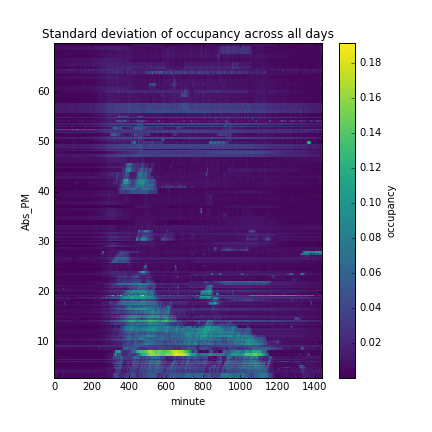
\includegraphics[scale=0.5]{../occ_sd.png}
    \caption{Occupancy varies more in areas of high traffic.}
\end{figure}

Figure~\ref{fig:occ_sd} shows the standard deviations of the difference
$y_{ijk}$. The bright line around mile 8 marks the toll plaza to enter
San Francisco. Lighter regions occur during the morning rush hour starting just
before 7 AM, and all along the area between mile markers 0 and 15 during
the day time, which corresponds to the area of high traffic between San
Francisco and Berkeley. This shows that occupancy exhibits significant
variablility in regions of congested traffic. The implication for this
analysis is that the difference $y_{ijk}$ will have more noise in these
regions, which makes it more difficult to accurately detect traffic events
of high occupancy.

\begin{figure}
    \label{fig:diffs}
    \centering
    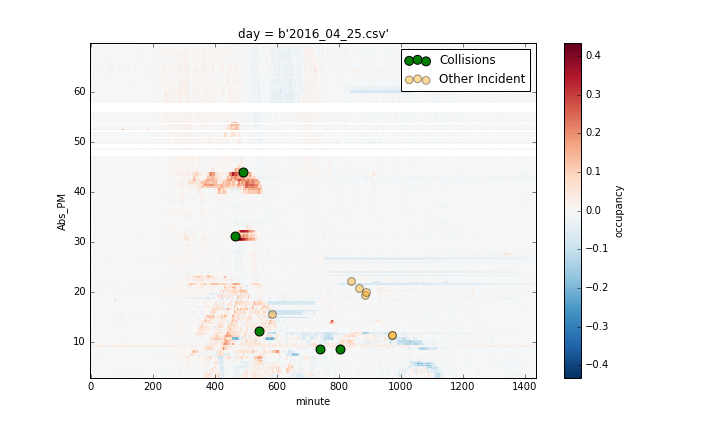
\includegraphics[scale=0.5]{../diffs.png}
    \caption{This shows the difference in occupancy from the median. Areas
    of unusually high occupancy are colored dark red.
    }
\end{figure}

Figure~\ref{fig:diffs} displays the differences $y_{ijk}$ as defined in
equation~\ref{eq:diff} on April 25th.  Corresponding CHP incidents have
been plotted in the same graph.  Two areas of high occupancy exist around
minute 400, one at mile 30 and one just above mile 40. Since there are
green points representing collisions in these regions it seems reasonable to
associate the traffic event with CHP incident data.

Simple image processing techniques were used to isolate and quantify these areas of
high occupancy. The first step was to use simple thresholding to create a
new binary variable that flags every observation that's larger than a
certain size.
Mathematically, let $z_{ijk} = 1 if y_{ijk} > t$ and $z_{ijk} = 0 if y_{ijk}
\leq t$. Some experimentation showed $t = 0.1$ to be a reasonable threshold
value. This produces figure~\ref{fig:thresh}. This resulting variable
$z_{ijk}$ was
then treated as an image; shapes were inferred by finding bounding boxes
for connected components.

\begin{figure}
    \label{fig:thresh}
    \centering
    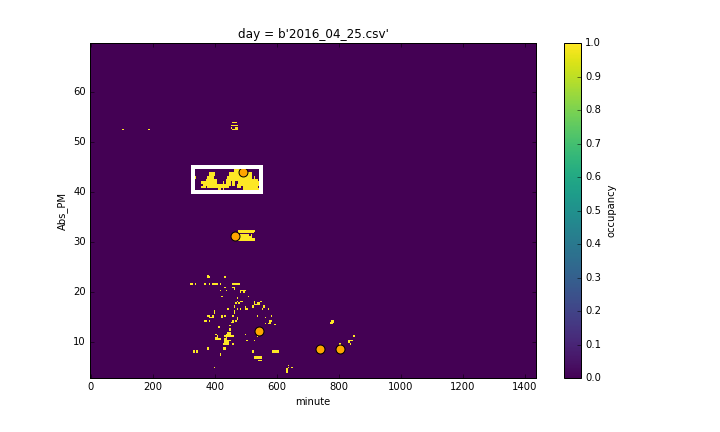
\includegraphics[scale=0.5]{../thresh.png}
    \caption{Areas of high occupancy have been converted to a binary
    variable.}
\end{figure}


Occupancy data was treated as an image. To compute the 

We can use opencv to do this. For each freeway we can take the following
steps:
\begin{enumerate}
    \item Read the raw file and convert it to an image with many missing
        values. 
    \item Interpolate missing values. 
    \item Threshold the image, so for a pixel with density $\rho >
        \rho_0$
        we define it as high density, otherwise low density. We'll
        have to experiment to see what the appropriate value of $\rho_0$ is
        but I suspect around 0.3.
    \item Once this has been done for every day we can compute an average
        thresholded image showing the areas of high density. This will show
        recurring bottlenecks. May need to threshold this also.
    \item Compare each day with the average. The difference will show the
        unusual patterns that occurred on just one day. Might have to do
        some denoising here- eliminate points that are not part of a 
        cluster.
\end{enumerate}

Once we have the denoised difference we can do the following:
\begin{enumerate}
    \item (Optional) Detect shapes that are flat on top, since this is the
        distinguishing feature of a bottleneck.
    \item Compute centroid, bounding boxes, and area which will quantify the impact
        in terms of space and time.
    \item Join these features to incident data. This likely will require some text
        analysis.
\end{enumerate}

Then we can answer questions such as:
\begin{enumerate}
    \item How many traffic events occur which have no associated incident
        data? And what sort of events were they probably?
    \item What is the impact of an event of type X on a given section of
        highway? Something along the lines of: When traffic flow is 1500
        veh per lane per hour in a two lane freeway a collision involving
        exactly two vehicles typically creates congestion lasting 10-15
        minutes which propagates back 2-3 miles. 
    \item How can we model the distribution of traffic incidents, ie.
        Poisson with some parameters.
\end{enumerate}

But how can these results be useful more broadly? More accurate
simulations. Input to real time routing. Impacts of planned construction
events. Scheduling CHP patrols and recovery services.

\section{Statistical Analysis}
%%%%%%%%%%%%%%%%%%%%%%%%%%%%%%%%%%%%%%%%%%%%%%%%%%%%%%%%%%%%

TODO: Clark will do this part

\section{Conclusions}
%%%%%%%%%%%%%%%%%%%%%%%%%%%%%%%%%%%%%%%%%%%%%%%%%%%%%%%%%%%%

TODO:

\bibliography{citations} 

\bibliographystyle{apalike}

\end{document}
